


\chapter{Numerical Results}
  \label{ch_results}

In his 1974 paper, Radoski argues that a poloidally-polarized wave should asymptotically rotate to the toroidal polarization\cite{radoski_1974} as a result of the curved derivative in the meridional plane. The question of finite poloidal lifetimes is considered further in a 1995 paper by Mann and Wright\cite{mann_1995}. Their numerical work used a straightened field line, with an \Alfven speed gradient in the ``radial'' direction. They also found a rotation over time from poloidal to toroidal polarization, with the characteristic time proportional to the azimuthal modenumber. 

\todo{Ding et al\cite{ding_1995} did similar work just before Mann and Wright, but results were less clear, possibly due to issues with grid resolution (as discussed in \cite{mann_1995}). }

\todo{Mann and Wright looked specifically at second harmonics. This work is on first harmonics. (In principle Tuna allows arbitrary driving waveforms and spatial distributions.) }

The present chapter builds on the aforementioned results by relaxing several of their nonphysical assumptions. Tuna's geometry (as described in \cref{ch_model}) is far more realistic than Radoski's half-cylinder or the box model used by Mann and Wright. Magnetic field lines are dipolar. \Alfven speed is based on an empirical profile, and varies along and across field lines. The present work also features driving delivered over time through perturbation of the ring current; past work has instead considered only the evolution of an initial condition. Finally, the present model includes a height-resolved ionosphere (rather than perfectly-reflecting boundaries). The ionospheric conductivity provides a direct coupling between the poloidal and toroidal modes, in addition to dissipating energy. 

\todo{We look at the interplay between poloidal-to-toroidal rotation, Joule dissipation, etc. }

%\todo{Do we every check E/B against $\Sigma_P / \mz$? }

%\todo{Do we see a difference between \vec{k} (momentum) and the group velocity? Poynting flux will always be pretty much along the field line, since $B_3$ is small and $E_3$ is zero, but the wave vector need not be. This is a question of coupling/converting to compressional waves, I guess. }

%\todo{Look at McKenzie and Westphal. Waves incident on the bow shock, etc, at weird angles. }

%\todo{Look at the E to B ratio. Compare to the \Alfven speed and to the height-integrated Pedersen conductivity. }

% -----------------------------------------------------------------------------
% -----------------------------------------------------------------------------
% -----------------------------------------------------------------------------
\section{Modenumber and Compressional Coupling}
  \label{sec_compression}

\todo{The overarching motivation for this work is that Pc4 pulsations vary in interesting ways with respect to azimuthal modenumber, and that prior models have been unable to give a good picture of that behavior. }

The fact that the poloidal mode is compressional at low modenumber, but not at high modenumber, is well known. However, the relationship is not well quantified. Theoretical work has historically been focused on the limits $\azm \rightarrow 0$ and $\azm \rightarrow \infty$\cite{cummings_1969,radoski_1974}, and only a handful of satellite observations have explicitly considered an event's azimuthal modenumber\cite{dai_2013,motoba_2015,takahashi_2013}. 

\cref{fig_snapshot_smallm,fig_snapshot_bigm} show magnetic field snapshots taken from a run with small \azm and a run with large \azm. These runs were performed using the quiet dayside ionospheric profile, but other profiles produce qualitatively similar results. The differences between the profiles are explored in \cref{sec_day,sec_night}. The two runs shown are identical except for the modenumber: same driving, same physical parameter profiles, etc. 

\todo{Morphology is qualitatively the same for all ionospheric profiles. Poloidal modes are spread broadly in $L$. Toroidal modes are sharp. Higher harmonics show up at large $L$. The differences between the profiles are explored in \cref{sec_day,sec_night}. }

\begin{figure}[!htb]
    \centering
    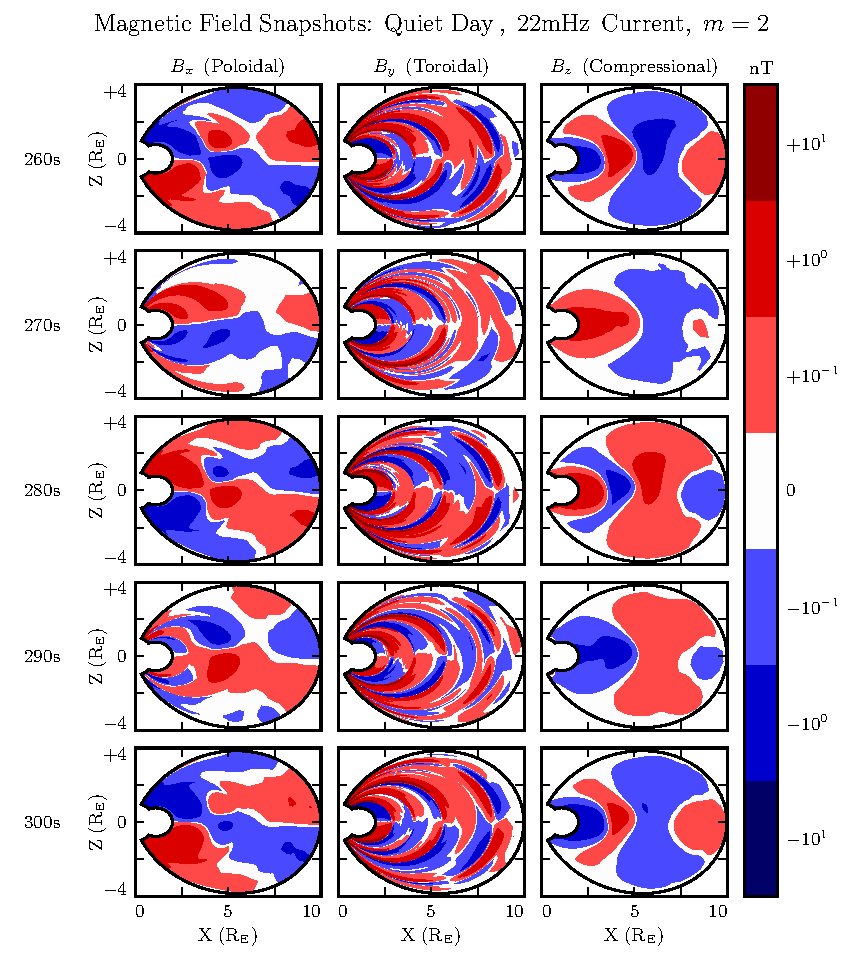
\includegraphics[width=\textwidth]{figures/snapshot_smallm.pdf}
    \caption[Magnetic Field Snapshots from a Small-\azm Run]{
      \todo{$\cdots$}
    }
    \label{fig_snapshot_smallm}
\end{figure}

\begin{figure}[!htb]
    \centering
    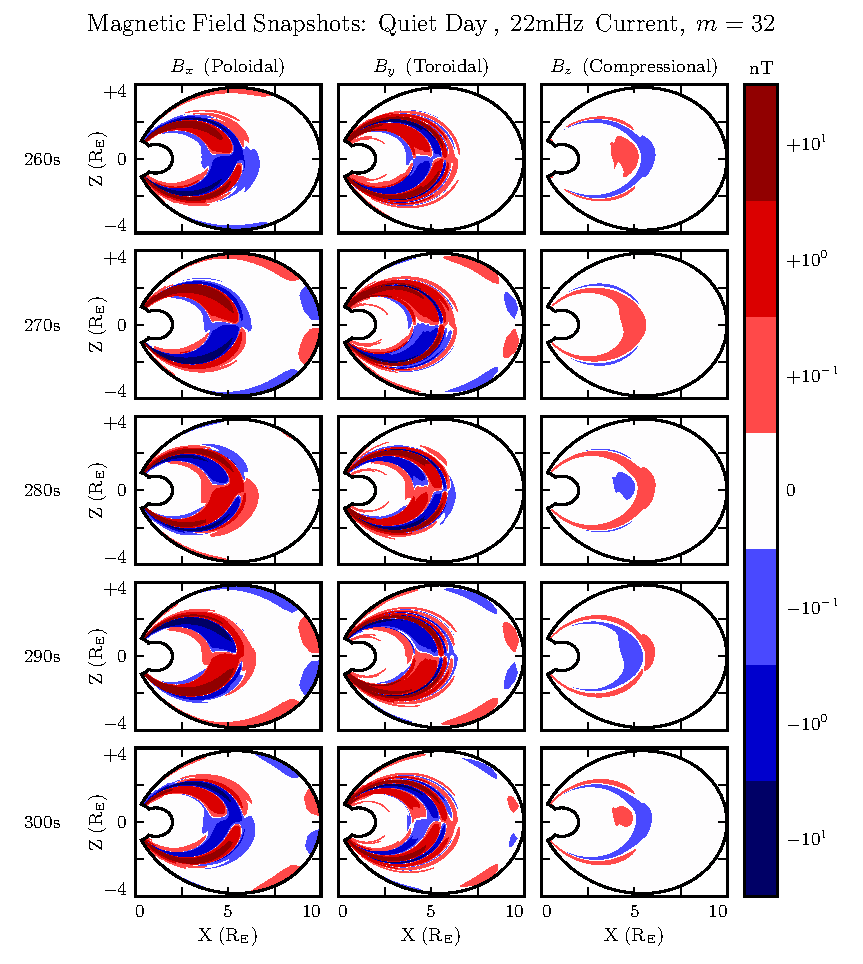
\includegraphics[width=\textwidth]{figures/snapshot_bigm.pdf}
    \caption[Magnetic Field Snapshots from a Large-\azm Run]{
      \todo{$\cdots$}
    }
    \label{fig_snapshot_bigm}
\end{figure}

\cref{fig_comp_2} shows the ratio of the compressional magnetic field to the poloidal magnetic field for an ensemble of runs, including those shown in \cref{fig_snapshot_smallm,fig_snapshot_bigm}. RMS field values are used, integrating over the volume of the simulation. Dotted lines indicate the mean, which is also listed at the top of each subplot. 

\todo{Sawtooth shape --- the compressional magnetic field is pumped up by the driving, but drops quickly since compressional propagation is evanescent. }

\todo{There's a bit of frequency dependence in the compressional coupling. Higher-frequency runs are more compressional. This is presumably because higher-frequency runs are closer to the compressional cutoff, so they are not quite as evanescent in the compressional direction. }

\todo{Results might vary significantly for even modes. Radoski's 1974 paper suggests that $\left|\frac{B_z}{B_x}\right|\sim\frac{1}{n}$ (where $n$ is the harmonic number). }

\begin{figure}[!htb]
    \centering
    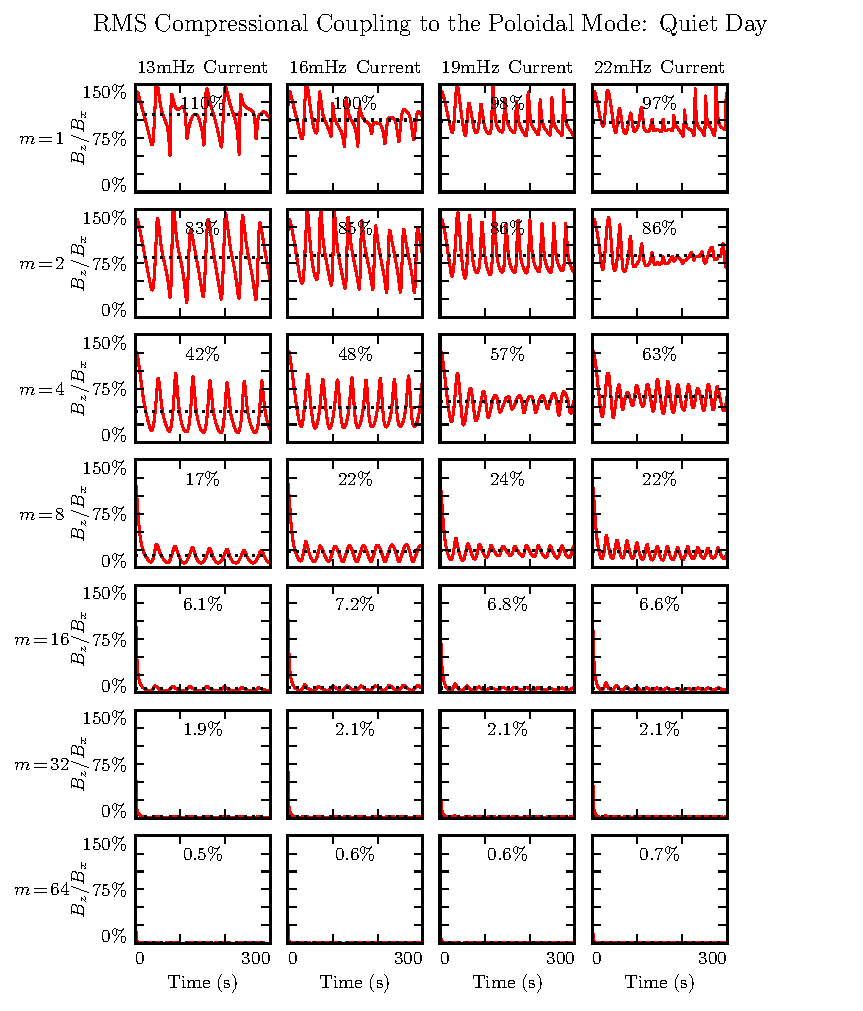
\includegraphics[width=\textwidth]{figures/comp_2.pdf}
    \caption[Compressional Coupling to the Poloidal Mode]{
      \todo{By varying the frequency and ionospheric profiles, the coupling at $\azm > 16$ can change by as much as a factor of two. But everything still converges to zero. }
    }
    \label{fig_comp_2}
\end{figure}

At $\azm = 1$, when the cutoff frequency\footnote{See \cref{fig_cutoff}. } is well below the drive frequency, the compressional and poloidal wave magnetic fields are (on average) equally strong. As \azm increases, the poloidal mode's compressional propagation becomes constrained, and the compressional magnetic field weakens. The compressional magnetic field's relative magnitude is cut in half by $\azm\about5$ (for non-quiet-night profiles), and cut in half again by $\azm\about10$. (Using the quiet night profile, the strength is instead halved at $\azm\about7$ and quartered at $\azm\about14$). 

\todo{The nature of the relationship between \azm and the compressional coupling is not obvious. It's not linear, logarithmic, or a power law. }

\todo{These results line up nicely with Dai's 2015 survey of poloidal Pc4 events\cite{dai_2015}. Events are characterized as compressional or non-compressional based on the ratio $\left|\frac{B_z}{B_x}\right|$. The threshold is arbitrarily set to \num{0.2} --- with no suggestion of a corresponding value of \azm. The results in \cref{fig_comp_2} suggest that Dai's threshold (conveniently!) aligns closely with the paper's definition of ``small \azm'' to mean $\azm < 10$. }

\todo{Check if a relationship is given in Hughes\cite{hughes_1994}. That's what Lei cites for ``low-\azm waves are compressional.'' Other papers give no indication that this has been looked at before\cite{cummings_1969,radoski_1974}. }

% -----------------------------------------------------------------------------
% -----------------------------------------------------------------------------
% -----------------------------------------------------------------------------
\section{Resonance and Rotation on the Dayside}
  \label{sec_day}

Each subplot in \todo{$\cdots$} is analogous to Figure 3 in Mann and Wright's paper\cite{mann_1995}. Blue lines show the total energy in the poloidal mode as a function of time. Red lines show toroidal energy. Runs are organized such that driving frequency is constant down each column, and azimuthal modenumer is constant across each row. Axis bounds are held constant across all subplots. 

The 28 runs shown in \todo{$\cdots$} use a high-conductivity profile, corresponding to the dayside with low solar activity (shown in \cref{sec_profile}). The two dayside profiles --- active and quiet --- are contrasted briefly in \cref{sec_ground}. However, the primary focus is on the difference between the dayside and the nightside. The differences between the two dayside profiles are minor in comparison. 

The fact that red (toroidal) lines appear at all speaks to the coupling of the poloidal and toroidal modes. As discussed in \cref{sec_driving}, driving in Tuna is delivered purely into the poloidal electric field (reflecting the azimuthal direction of the ring current). 

As expected, the rotation from poloidal to toroidal is slowest at large azimuthal modenumbers. The toroidal energy overtakes the poloidal energy within a single drive period at $\azm=4$; at $\azm=64$, the most of the energy is in the poloidal mode for \about10 periods. However, the relationship between azimuthal modenumber and rotation timescale is not linear, as was suggested by Mann and Wright. Instead, the rotation is fastest at $\azm=4$. 

This hints at two competing effects, and there are only so many options. In addition to the poloidal-to-toroidal rotation, the two modes are coupled by the ionospheric Hall conductivity; energy is also is lost when waves propagate out of the simulation domain, when driving interferes destructively with a wave, and as a result of Joule dissipation. 

In practice, the Hall conductivity does not move large amounts of energy between the poloidal and toroidal modes. In fact, when the runs shown in \todo{$\cdots$} are repeated with Hall conductivity uniformly zero (not shown), the energy curves do not change appreciably. 

Joule dissipation --- a recurring topic in the present chapter --- is a major player in the simulation's energy economy, but does not depend directly on the azimuthal modenumber. Similarly, azimuthal modenumber does not immediately impact the interference between a wave and its driver. 

That leaves the propagation of energy across field lines, which does explain the observed behavior. As the azimuthal modenumber increases past order unity, compressional \Alfven waves in the Pc4 band become evanescent\footnote{See \cref{sec_implications}. }. Runs in the top two rows lose considerable sums of energy as a result of waves propagating out of the simulation domain. In contrast, runs conducted at higher modenumber do not permit the compressional propagation of \Alfven waves, so energy does not escape through the outer boundary. 

Notably, the low-modenumber runs at \SI{19}{\mHz} do accumulate significant energy over time, while those at \SI{13}{\mHz}, \SI{16}{\mHz}, and \SI{22}{\mHz} falter. This response is likely nonphysical, and is discussed in \todo{$\cdots$}. 

In each run, the energy of the system is asymptotically determined by the balance between the energy input (from driving) and the energy loss (through Joule dissipation in the ionosphere and escape through the boundary). When the driving frequency matches closely with the local \Alfven frequency, energy accumulates over a number of drive periods, leading to a relatively large asymptotic energy in the system. 

%The system's resonant frequency (for a fundamental poloidal mode at $L\about5$) is affected significantly by the size of the plasmasphere. In \cref{fig_U_2_4_5}, with the plasmapause at $L_{PP}=4$, the system resonates at \SI{19}{\mHz} at low \azm; as \azm becomes large, the resonant frequency is closer to \SI{22}{\mHz}. \cref{fig_U_2_5_5} shows the effect of moving the plasmapause to $L_{PP}=5$: resonance is closer to \SI{16}{\mHz}. The runs are otherwise identical to those shown in \cref{fig_U_2_4_5}. 

\todo{In most cases, the energy in the toroidal mode exceeds the energy in the poloidal mode. }

\todo{The late, long dips in energy are probably due to ``beats'' in the interference between the driving frequency and the bounce frequency. }

Looking a bit deeper, it's possible to comment on the structure of the poloidal and toroidal modes, not just their magnitudes. The subplots in \todo{$\cdots$} are arranged analogously to those in \todo{$\cdots$}: each comes from a different run, modenumber is held constant across each row, and frequency down each column. 

Contours represent energy density, averaged over the volume of a flux tube. The vertical axis shows $L$-shell, while the horizontal axis is time. As above, poloidal and toroidal energy density are computed separately. 

\todo{$\cdots$} shows why, at low modenumber, the poloidal mode does not resonate well. Its compressional component allows energy to be spread broadly in $L$ --- in fact, at $\azm = 1$, no energy buildup at all is apparent at the location of the driving. 

Some energy moves inward, and is trapped in the plasmapause's steep \Alfven speed gradient (particularly visible in the \SI{16}{\mHz}, $\azm = 4$ run). Some energy builds up in a third harmonic resonance near the outer boundary (shown best in runs with $\azm = 1$). The time spent propagating across field lines counts against the poloidal mode's finite lifetime --- by the time a poloidally-polarized wave reaches the outer boundary, a significant fraction of its energy has rotated to the toroidal mode. 

It's likely that at \SI{19}{\mHz}, with $\azm = 1$, the response is artificially amplified through interaction with the boundary conditions. As mentioned in \cref{sec_bcs}, nonphysical reflections can occur when waves are very close to the boundary. In most cases, waves are not localized at the boundary, so this is not a concern. 

The peak energy density in the bottom-right run (\SI{22}{\mHz} driving, $\azm = 64$) is by far the largest of any run in \todo{$\cdots$}. The azimuthal modenumber is large, so the poloidal mode is purely guided; no time is wasted with movement across magnetic field lines. And, crucially, the frequency of the driving aligns closely with the resonant frequency where it's delivered. Other runs on the bottom row also have $\azm = 64$ (and so are also guided), but their driving frequencies do not align with the local resonant frequency. As a result, they do not accumulate energy over a large number of drive periods. 

%Similar behavior can be seen in \todo{$\cdots$} (which shows the same runs as \todo{$\cdots$}, with the plasmapause moved to $L_{PP} = 5$ from its default location at $L_{PP} = 4$). A third harmonic resonance can be seen at the outer boundary for runs on the top row ($\azm = 1$). The effect of the plasmapause is particularly visible in the middle row, $\azm = 8$, where energy accumulates both just inside and just outside $L_{PP} = 5$. At high modenumber, the driving resonates best at \SI{16}{\mHz}; at other frequencies, energy density has a lower asymptotic value, which is reached more quickly. 

In \todo{$\cdots$}, the poloidal contours show energy smeared across a swath of $L$-shells. On the other hand --- as shown in \todo{$\cdots$} --- the toroidal mode appears only where the drive frequency matches the local eigenfrequency. 

A horizontal line drawn through the \Alfven speed frequency profiles (recall \cref{fig_fa}) intersects the profile up to three times: once as the \Alfven frequency drops through the Pc4 range from its low-latitude peak, again as the \Alfven frequency rises sharply at the plasmapause, and a third time as the \Alfven frequency drops asymptotically. Toroidal waves can be seen resonating at all three of these locations in the $\azm = 4$, \SI{19}{\mHz} run in \todo{$\cdots$}, along with a third harmonic at large $L$. 

This is consistent with observations: toroidal resonances are noted for having frequencies which depend strongly on $L$, in contrast to the poloidal mode's less-strict relationship between frequency and location. 

The dayside poloidal modes shown in \todo{$\cdots$} attain an energy density on the order of \SI{e-1}{\nJ/\meter\cubed} only under ideal conditions: high modenumber runs with driving close to the local \Alfven frequency. Between the 56 dayside runs shown, such energy density appears only twice. On the other hand, the toroidal mode reaches \about\SI{e-1}{\nJ/\meter\cubed} in six of the runs in \todo{$\cdots$} alone. That is, the poloidal mode only exhibits a high energy density on the dayside only when conditions are ideal; the toroidal mode isn't nearly so particular. 


Each subplot above corresponds to a \SI{300}{\s} run of Tuna, driven in the poloidal mode. At low \azm, energy instead moves radially and rotates quickly to the toroidal mode, precluding the formation of poloidal FLRs. At high \azm, the poloidal mode is guided, and the mode rotation is slow, allowing a strong resonance --- but only when the driving frequency matches the local \Alfven frequency. 

The \Alfven frequency profile is significantly affected by the size of the plasmasphere. The runs shown above are identical to those in \cref{fig_layers_p_2_4_5}, except that the plasmapause has been moved from $L_{PP} = 4$ to $L_{PP} = 5$. As a result, the most effective resonance at $L\about5$ is shifted from \SI{22}{\mHz} to \SI{16}{\mHz}. 

On the dayside, energy accumulates in the toroidal mode only at $L$ values where the drive frequency matches a local eigenfrequency. This is in contrast to the more smeared appearance of the poloidal contours shown in \cref{fig_layers_p_2_4_5,fig_layers_p_2_5_5}. Furthermore, the toroidal mode attains a high energy density under more diverse conditions than the poloidal mode. 

Ionospheric conductivity on the dayside is high. 

Energy is computed per Poynting's theorem, with due consideration of the unusual geometry. Energy density is integrated over the meridional plane, but not in the azimuthal direction, giving units of gigajoules per radian; more than anything else, this serves as a reminder that the waves under consideration are azimuthally localized. The energy in the poloidal mode and the energy in the toroidal mode are, respectively, 
\begin{align}
  \label{def_energy}
  U_P &= \displaystyle\int \frac{d\lysakx d\lysakz}{2 \mz \jac} \lr{ B_x^2 + \frac{1}{\va^2} E_y^2} &
  U_T &= \displaystyle\int \frac{d\lysakx d\lysakz}{2 \mz \jac} \lr{ B_y^2 + \frac{1}{\va^2} E_x^2} 
\end{align}


Each subplot in \cref{fig_U_day,fig_layers_day_p,fig_layers_day_t} corresponds to a run. 


\begin{figure}[!htb]
    \centering
    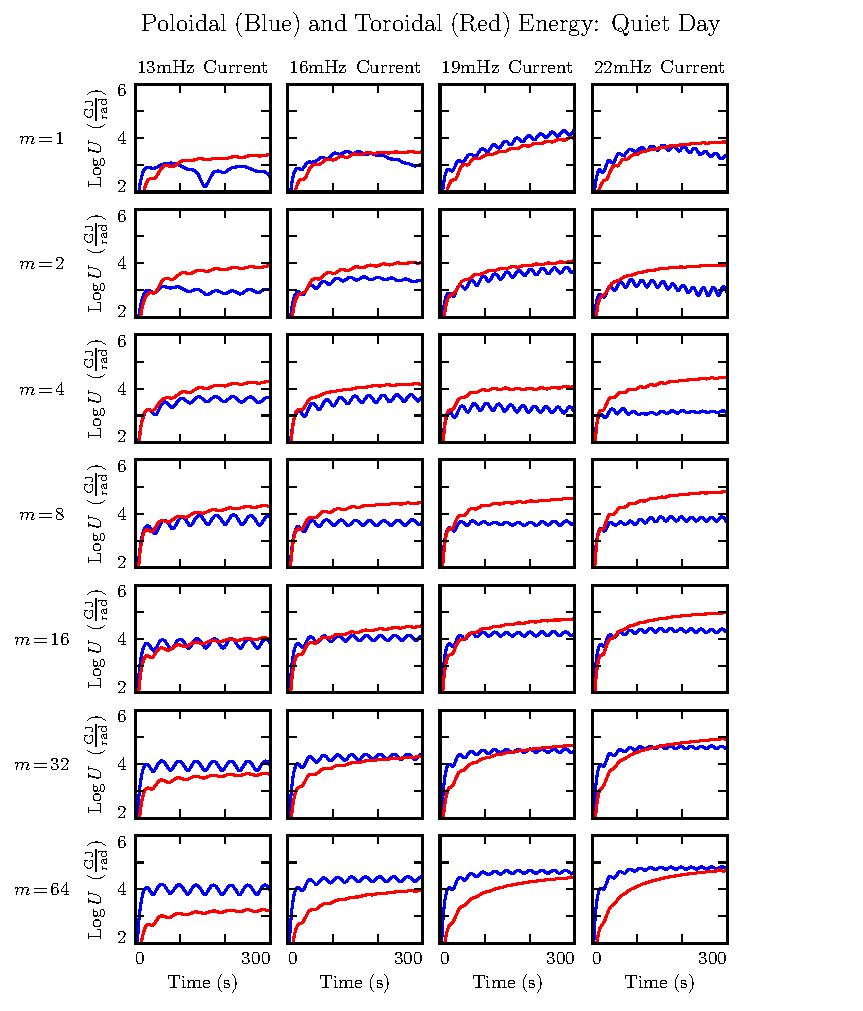
\includegraphics[width=\textwidth]{figures/U_day.pdf}
    \caption[Dayside Poloidal and Toroidal Energy]{
      \todo{$\cdots$}
    }
    \label{fig_U_day}
\end{figure}


\begin{figure}[!htb]
    \centering
    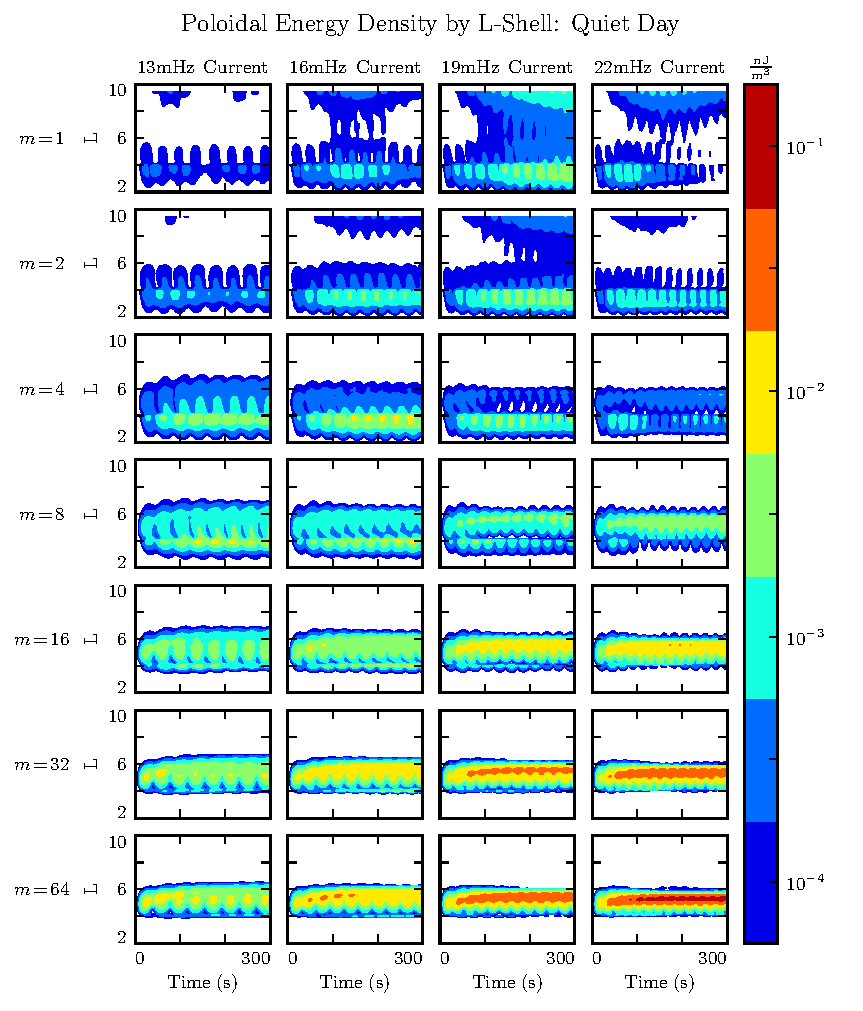
\includegraphics[width=\textwidth]{figures/layers_day_p.pdf}
    \caption[Dayside Poloidal Energy Distribution]{
      \todo{$\cdots$}
    }
    \label{fig_layers_day_p}
\end{figure}

\begin{figure}[!htb]
    \centering
    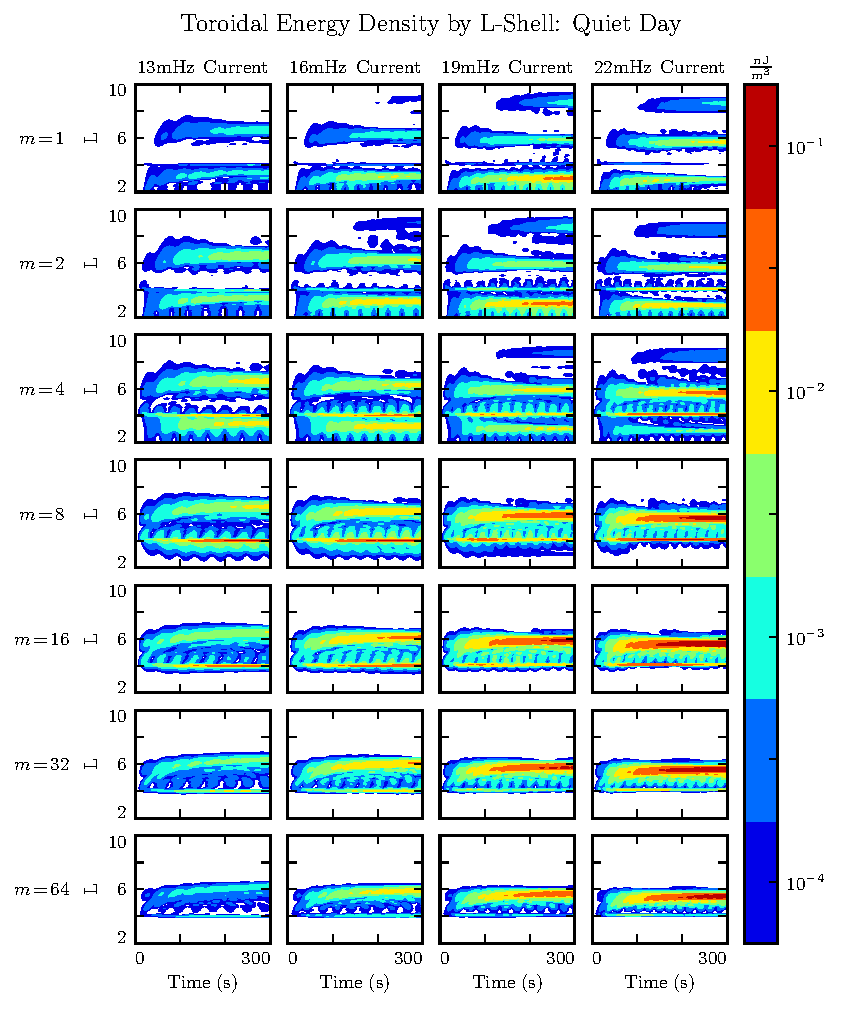
\includegraphics[width=\textwidth]{figures/layers_day_t.pdf}
    \caption[Dayside Toroidal Energy Distribution]{
      \todo{$\cdots$}
    }
    \label{fig_layers_day_t}
\end{figure}

% -----------------------------------------------------------------------------
% -----------------------------------------------------------------------------
% -----------------------------------------------------------------------------
\section{Resonance and Rotation on the Nightside}
  \label{sec_night}

Each subplot in \cref{fig_U_night,fig_layers_night_p,fig_layers_night_t} corresponds to a run. 

Driving is moved from $L=5$ to $L=6$ to line up better. Or even $L=7$?


\begin{figure}[!htb]
    \centering
    
\includegraphics[width=\textwidth]{figures/placeholder.jpg}
    \caption[Nightside Poloidal and Toroidal Energy]{
      \todo{$\cdots$}
    }
    \label{fig_U_night}
\end{figure}


\begin{figure}[!htb]
    \centering
    
\includegraphics[width=\textwidth]{figures/placeholder.jpg}
    \caption[Nightside Poloidal Energy Distribution]{
      \todo{$\cdots$}
    }
    \label{fig_layers_night_p}
\end{figure}

\begin{figure}[!htb]
    \centering
    
\includegraphics[width=\textwidth]{figures/placeholder.jpg}
    \caption[Nightside Toroidal Energy Distribution]{
      \todo{$\cdots$}
    }
    \label{fig_layers_night_t}
\end{figure}



Compared to the dayside ionosphere employed in \cref{sec_day}, the nightside profiles exhibit two major differences. The ionospheric conductivity is lower, and the \Alfven speed is higher. The present section and \cref{sec_layers_night} show results using only the active nightside profile. The differences between the quiet and active nightside ionospheric profiles are small compared to the differences between either dayside profile and either nightside profile; all four profiles are briefly compared in \cref{sec_ground}. 

The low conductivity on the nightside gives rise to strong Joule dissipation. Waves are damped out in just a few bounces, so asymptotic energy values are reached quickly. Even so, the poloidal-to-toroidal rotation is qualitatively the same as on the dayside. The further the azimuthal modenumber from the rotation peak at $\azm = 4$, the lower the asymptotic toroidal energy level is compared to the poloidal. If anything, the effect is exaggerated by the small dissipation timescale. When $\azm = 64$, no more than \about\SI{10}{\percent} of the energy in the poloidal mode rotates to the toroidal mode before being lost. 

\todo{$\cdots$} is arranged analogously to the figures in \cref{sec_day}: each subplot is an independent run, drive frequency is constant down each column, and azimuthal modenumber is constant across each row. Poloidal energy is blue; toroidal energy is red. 

The lower energies in \todo{$\cdots$} (compared to \todo{$\cdots$}, the analogous dayside runs) are not entirely due to increased Joule dissipation. Due to the difference in electric constant between the dayside and nightside magnetospheres\footnote{See \cref{fig_fa}. }, resonant frequencies just outside the typical ($L_{PP} = 4$) plasmapause fall well outside the Pc4 range. None of the frequencies shown in \todo{$\cdots$}, when delivered at $L_{drive} = 5$, align with the local eigenfrequency. 

As in \todo{$\cdots$}, the \SI{19}{\mHz} run with $\azm = 1$ is an apparent exception. A large amount of energy builds up in a third harmonic very close to the outer boundary. The interaction is likely nonphysical. 

\todo{It may be significant that $\int \sigma dz$ is constant across all $L$-shells, but $\int \frac{\sigma}{\va^2} dz$ is not. }

Behavior closer to resonance is shown in \todo{$\cdots$}. The plasmapause remains at $L_{PP} = 4$, but the driving is moved out to $L_{drive} = 6$, at which point the local \Alfven frequency overlaps the Pc4 frequency band. 

There is surprisingly little difference between \todo{$\cdots$} (the subplots of which are arranged analogously). Asymptotic energy levels vary --- in the case of high \azm and low frequency, runs in \todo{$\cdots$} are more energetic by an order of magnitude or more --- but the qualitative behavior is the same. Driving is balanced by dissipation over the course of just a few drive periods. Dissipation outstrips poloidal-to-toroidal rotation in the case of large azimuthal modenumber. And, unlike on the dayside, the toroidal mode typically does not match the asymptotic energy level seen in the poloidal mode. 

\todo{$\cdots$} shows the radial distribution of poloidal energy on the nightside --- a slice of each run shown in \todo{$\cdots$}. Broadly speaking, the behavior is consistent with that seen in \todo{$\cdots$}: energy is smeared across $L$-shells at small \azm and guided at high \azm, with particularly strong energy buildup when the drive frequency matches the local \Alfven frequency. 

As discussed in \todo{$\cdots$}, the nightside's relatively low ionospheric conductivity increases the rate of dissipation. Asymptotic energy content is reached quickly, and is small compared to that seen in analogous dayside runs. 

The effect is particularly pronounced at large modenumber, where the poloidal-to-toroidal rotation timescale is slower than the nightside dissipation timescale. In most of the dayside runs shown in \todo{$\cdots$}, the toroidal mode asymptotically exceeds the poloidal mode both in terms of total energy content and in terms of peak energy density. On the nightside, the opposite is true. At high modenumber, the asymptotic rotation from the poloidal mode to the toroidal mode doesn't occur until most of the energy has been lost to Joule dissipation. Peak poloidal energy densities at $\azm = 64$ exceed their toroidal counterparts --- shown in \todo{$\cdots$} --- by an order of magnitude. 

\todo{On the nightside, unlike the dayside, toroidal contours are messy. Why? }

The behavior of the poloidal mode on the nightside matches qualitatively with the behavior on the dayside. At low \azm, energy is lost to the outer boundary. At high \azm, resonance occurs, but only if the drive frequency is close to the local eigenfrequency. The big difference is that, due to the increased dissipation in the ionopshere, asymptotic energy densities are relatively low, and reached relatively quickly. 

In low-\azm runs, the poloidal mode loses energy to the outer boundary, which impairs the growth of the toroidal mode. At high \azm, poloidal-to-toroidal rotation is slow compared to dissipative timescales on the nightside. The strongest toroidal waves --- which are still weak compared to those on the dayside --- thus appear at moderate \azm. 









% -----------------------------------------------------------------------------
% -----------------------------------------------------------------------------
% -----------------------------------------------------------------------------
\section{Ground Signatures and Giant Pulsations}
  \label{sec_ground}

While the majority of the action is in space, the majority of FLR observations have been ground-based. The present section explores the same simulations discussed in \cref{sec_lifetimes_day,sec_layers_day,sec_lifetimes_night,sec_layers_night}, but in terms of their ground signatures rather than their broad energy distributions. 

As in the figures shown in \cref{sec_lifetimes_day,sec_layers_day,sec_lifetimes_night,sec_layers_night}, each row in \cref{fig_ground_day,fig_ground_night} shows runs at a different modenumber. The columns are magnetic field contours; the vertical axis is latitude, and the horizontal axis is time. The four columns are components of the magnetic field signatures at the ground:  the north-south magnetic field (first and third columns) and the east-west magnetic field (second and fourth columns). The pair on the left show a simulation carried out using the active ionospheric profile, and the pair on the right show a simulation using the quiet profile. 

Notably, the magnetic polarization of a low frequency \Alfven wave is rotated by \about\SI{90}{\degree} as it passes through the ionosphere\cite{hughes_1974}. The east-west field on the ground ($B_\phi$) corresponds to the poloidal polarization in space, and the north-south field on the ground ($B_\theta$) corresponds to the toroidal mode. 

\todo{What's going on with the empty frame for nightside, $\azm = 1$, \SI{16}{\mHz}? }

\todo{Don't use \SI{19}{\mHz}! It's wonky at low modenumber. Use \SI{22}{\mHz} instead. }

The most striking feature of \cref{fig_ground_day,fig_ground_night} is the modenumber dependence. As modenumber increases, the magnetic field signatures become sharply localized in latitude. At high \azm, ground signatures are concentrated between \SI{60}{\degree} and \SI{70}{\degree}, peaking just below \SI{65}{\degree}. This shows good agreement with observations of Pgs peaked near \SI{66}{\degree}. 

At low modenumber, magnetic signatures are weak on the ground because the waves in space are also weak. At high modenumber, waves in space are strong, but so is the attenuation of magnetic signatures by the ionosphere\footnote{See \cref{attenuation}. }. The ``sweet spot'' at which magnetic ground signatures are maximized falls at $\azm = 16$ to $\azm = 32$. For comparison, Pgs are generally observed with azimuthal modenumbers of 16 to 35\cite{takahashi_1992}. 

Ground signatures are maximized at $\azm = 16$ and $\azm = 32$ on both the dayside (\cref{fig_ground_day}) and the nightside (\cref{fig_ground_night}). Dayside signatures are stronger than those on the nightside, and quiet dayside and quiet nightside responses are stronger than those on the active dayside and active nightside respectively. The strongest magnetic fields at the ground are primarily east-west polarized -- as Pgs are\cite{takahashi_1992}. 

\todo{At present, Tuna's ionospheric profiles do not allow the dawn and dusk flanks to be distinguished from the dayside and nightside. }

\begin{figure}[!htb]
    \centering
    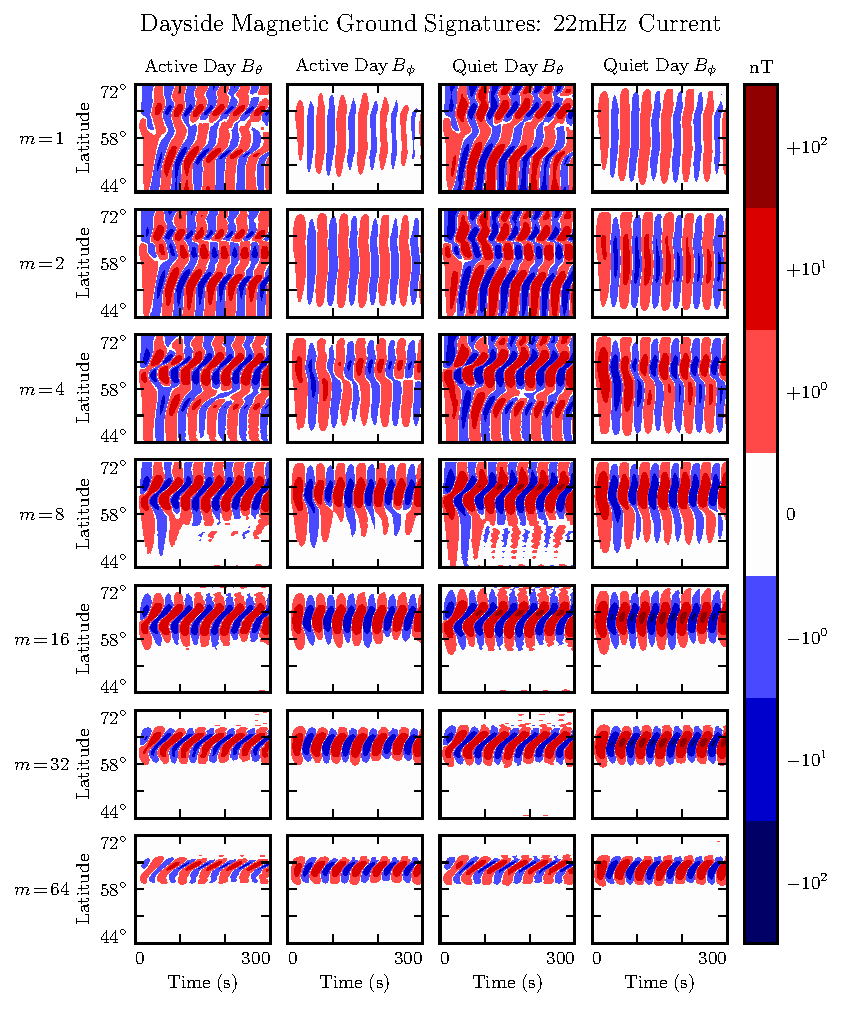
\includegraphics[width=\textwidth]{figures/ground_day.pdf}
    \caption[Dayside Ground Magnetic Fields]{
      \todo{$\cdots$}
    }
    \label{fig_ground_day}
\end{figure}

\begin{figure}[!htb]
    \centering
    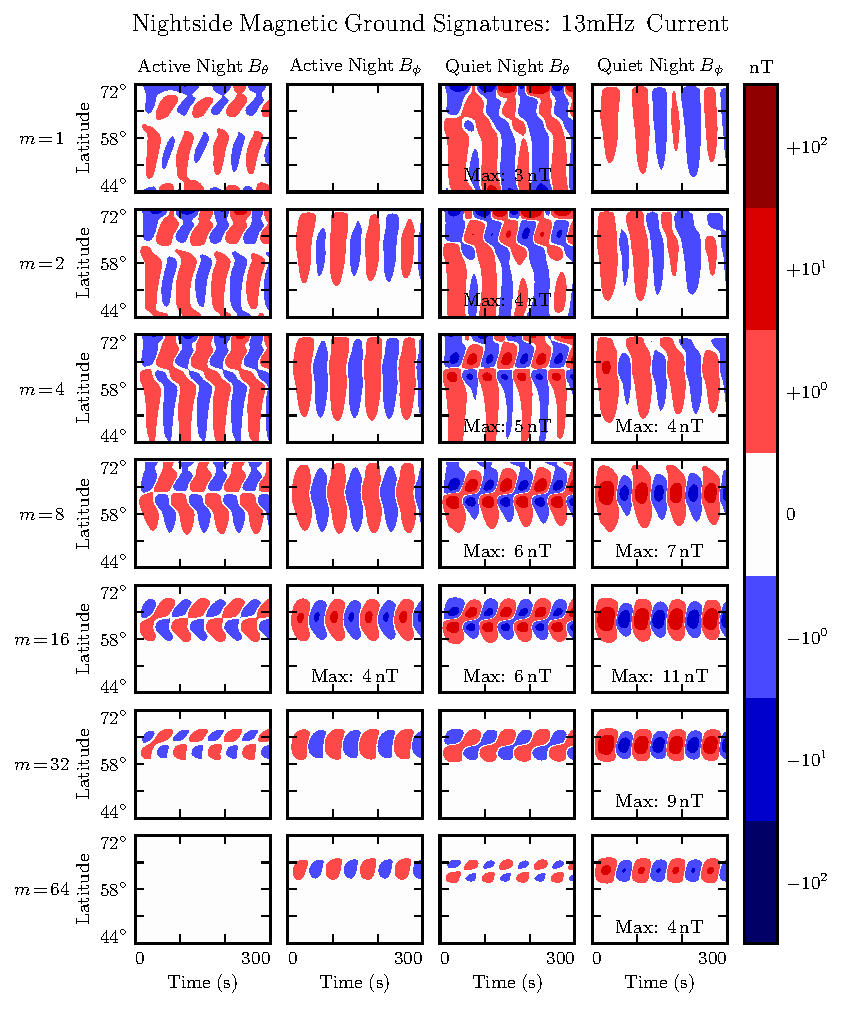
\includegraphics[width=\textwidth]{figures/ground_night.pdf}
    \caption[Nightside Ground Magnetic Fields]{
      Nightside ground signatures are less strongly peaked than those on the dayside, but qualitative features are the same: the strongest signals are in $B_\phi$, peaked over just a few degrees in latitude, at a modenumber of 16 or 32, under quiet ionospheric conditions. 
    }
    \label{fig_ground_night}
\end{figure}

% -----------------------------------------------------------------------------
% -----------------------------------------------------------------------------
% -----------------------------------------------------------------------------
\section{Discussion}

\todo{Make this section read nicely. }

%The results of the present section show agreement with --- and significant refinement of --- past analytical and numerical work. In the case of large (but finite) ionospheric conductivity, dipole geometry, and realistic \Alfven speed profile, energy rotates asymptotically from the poloidal mode to the toroidal mode. The rotation rate is strongly affected by azimuthal modenumber and, in the large-\azm regime, has a characteristic timescale in the tens of periods. 

%The present work furthermore considers the issue of poloidal lifetimes in the low conductivity regime (while past work has used perfectly-reflecting boundaries). Results show that an equally-strong driving current will create weaker FLRs on the nightside. 

%LIFETIMES

Poloidal FLRs rotate to the toroidal mode over time. Toroidal modes do not appear to rotate back to the poloidal mode. When \azm is small, the rotation is comparable to an oscillation period; when \azm is large, rotation timescales are comparable to ten periods, sometimes more.

On the dayside, little damping takes place over rotation timescales, so the toroidal mode asymptotically exceeds the toroidal mode. The exception is waves with low modenumber, where poloidal waves can escape by propagating across field lines. An evaluation of what happens then --- whether they bounce back off the magnetopause, for example --- is beyond the scope of the present work. 

On the nightside, the conductivity of the ionosphere is low enough that damping timescales become comparable to oscillation timescales. Waves are weaker, since they are unable to accumulate energy over as many periods. High-\azm toroidal waves are particularly weak, since the dissipation timescale is faster than the poloidal-to-toroidal rotation timescale. 

Waves resonate best when the frequency of the driving matches the local eigenfrequency where it's delivered. The eigenfrequency is significantly affected by the size of the plasmasphere. 

%LAYERS

%Low-\azm poloidal modes are not inclined to resonate just outside the plasmapause, even if the driving frequency matches the local eigenfrequency. They slide --- \todo{up?} --- the effective potential surface formed by the sharp \Alfven speed gradient. Some energy accumulates as a third harmonic at large $L$, and some within the plasmapause. 

The poloidal mode, due to its compressional character, exhibits an energy profile which is smeared in $L$. The toroidal mode, on the other hand, forms sharp resonances where the drive frequency matches the local eigenfrequency. This may explain why the observed frequencies of poloidal waves depend weakly on $L$, while the frequencies of toroidal waves are strongly dependent on $L$. 

%GROUND SIGNATURES

At low \azm, ground signatures are weak because waves in space are weak because energy can easily escape through the simulation's outer boundary. At large \azm, ground signatures are attenuated by the ionosphere. The ``sweet spot'' in azimuthal modenumber at which ground signatures are strongest is around 16 to 32. Furthermore, ground signatures are strongest when ionospheric profiles corresponding to solar minimum are used. Driving in the poloidal electric field gives rise to primarily ground signatures polarized primarily in the east-west direction at the ground. And, when the frequency of the driving does not match the local eigenfrequency, the high-\azm resonates weakly in place, rather than tunneling across field lines to resonate strongly somewhere else. 

These findings imply, awkwardly, that the morphology of giant pulsations may reveal relatively little about their origins. One can consider a hypothetical magnetosphere subject to constant driving: broadband in frequency, broadband in modenumber, just outside the plasmapause. Low-\azm poloidal waves will quickly rotate to the toroidal mode (and/or propagate away). High-\azm waves will resonate in place, accumulating energy over time, and giving rise to ``multiharmonic toroidal waves''\cite{takahashi_2011}; Fourier components that do not match the local eigenfrequency will quickly asymptote. Waves with very high modenumbers will be attenuated by the ionosphere. The response on the ground will be significantly stronger during quiet solar conditions. In other words, the measurements on the ground will look very much like a giant pulsation. 

\todo{Notably, the present work offers no explanation as to Pgs' distinctive distribution in MLT! }

%\todo{If \azm is small, energy rotates to the toroidal mode too fast to form a poloidal resonance. If \azm is large, the \Alfven wave is guided, so it resonates only if the driving frequency lines up with the resonant frequency where it's applied. The result is just one big --- or perhaps even giant --- pulsation. If the driving lines up with a nearby field line, the toroidal mode goes crazy! Resonance inside the plasmasphere. Resonance at the plasmapause. Resonance at the driving location. And (weak) attempt at a higher harmonic further out. }

%\todo{When the driving frequency doesn't line up with the location where it's delivered, there's basically no response. There is no movement of energy to a resonant field line, so no energy can accumulate over the course of multiple rounds of driving. Even when not driven resonantly, the toroidal mode still makes the best of its situation. It steals what energy it can from the poloidal mode, carries it to the resonant $L$-shell, and gets to work. (In contrast, recall from \cref{fig_resonant_driving}, in this situation the poloidal mode just does not accumulate energy.) }

